\documentclass[12pt,letterpaper]{article}

\usepackage[margin=1in]{geometry}
\usepackage[T1]{fontenc}
\usepackage[utf8]{inputenc}
\usepackage{graphicx}
\usepackage{enumitem}
\usepackage{algorithm}
\usepackage{algpseudocode}
\usepackage{setspace}
\usepackage{parskip}
\usepackage{helvet}
\usepackage{textcomp}
\usepackage[hidelinks]{hyperref}

\renewcommand{\familydefault}{\sfdefault}
\renewcommand{\thesection}{\arabic{section}.}
\renewcommand{\thesubsection}{\thesection\arabic{subsection}.}

\setlength{\parindent}{0.25in}
\setlength{\parskip}{0.08in}
\setlength{\emergencystretch}{2em}
\setlist[itemize]{leftmargin=0.5in,itemsep=0.02in,topsep=0.02in}
\setlist[enumerate]{leftmargin=0.5in,itemsep=0.02in,topsep=0.02in}

\newcommand{\ProjectTitle}{\ldots\ldots\ldots\ldots\ldots}
\newcommand{\GroupMembers}{\ldots}
\newcommand{\Supervisors}{\ldots}
\newcommand{\ReportDate}{}

\begin{document}

\hypersetup{pageanchor=false}
\begin{titlepage}
\centering

{\LARGE\bfseries ENS 491-492 -- Graduation Project\par}
\vspace{0.2in}
{\LARGE\bfseries Final Report\par}

\vspace{1.15in}
{\Large\bfseries Project Title: \ProjectTitle\par}

\vspace{1.3in}
{\large\bfseries Group Members: \GroupMembers\par}
\vspace{0.25in}
{\large\bfseries Supervisor(s): \Supervisors\par}

\vspace{0.55in}
{\large\bfseries Date: \ReportDate\par}

\vfill

\includegraphics[width=2.1in]{sabanci_logo.png}
\end{titlepage}
\hypersetup{pageanchor=true}

\begin{itemize}
\item \textbf{ENS 491-492 Final Report \underline{must contain} the following sections (leave section titles unchanged).}
\item \textbf{\underline{You are required to write clearly and concisely}: The main body of the report (not including the Title Page, Appendix, and References) must be between \underline{20--25 pages}.}
\item \textbf{Project advisor may have additional requirements for the report.}
\end{itemize}

\section{EXECUTIVE SUMMARY}
This ongoing research investigates how a large language model can be fine-tuned to classify phishing websites while producing explanations that are grounded in observable webpage evidence. The central problem is not only whether a webpage is phishing or benign, but whether the model can justify its verdict using signals that a security analyst can inspect, such as URL structure, title-domain consistency, forms, credential fields, redirects, external resources, and other HTML-derived artifacts. The intended output is a constrained JSON response containing a verdict, confidence level, evidence items, and a short explanation, rather than an unconstrained natural-language rationale.

The project uses a supporting data pipeline to collect and normalize webpages from phishing feeds, benign website rankings, and live security-scan sources. This infrastructure is necessary because LLM fine-tuning requires consistent inputs and reliable supervision, but it is not the primary contribution. The research focus is the design of a fine-tuning dataset, prompt schema, evidence schema, and evaluation procedure for an explainable phishing classifier. The current experimental direction uses parameter-efficient fine-tuning of a compact multimodal-capable language model in text-only mode, using URL, page title, and engineered URL/HTML/metadata features as model-visible inputs.

Work completed so far includes webpage collection, feature extraction, dataset construction, train-only feature selection, and baseline feature analysis. Classical models and explanation tools such as SHAP, LIME, and EBM are used as diagnostic instruments to understand feature behavior, dataset bias, and evidence candidates; they are not treated as the final research result. The main expected outcome is a fine-tuned LLM that can produce valid, evidence-grounded, schema-compliant phishing classifications. The project is still in progress, and final claims will require evaluation on domain-grouped and time-aware splits, schema-validity metrics, grounded-evidence metrics, and classification metrics on held-out data.

\section{PROBLEM STATEMENT}
Phishing websites remain a persistent security problem because they exploit user trust and imitate legitimate online services. They frequently collect credentials, payment information, or personal data through pages that look familiar to users but are hosted on unrelated or compromised infrastructure. The Anti-Phishing Working Group reported 853,244 phishing attacks in the fourth quarter of 2025 and 3.8 million attacks during 2025, with Social Media and SaaS/Webmail among the most frequently targeted sectors \cite{apwg2025q4}. These attacks are difficult to handle with static defenses alone because phishing pages are short-lived, change quickly, and often reuse legitimate-looking assets.

The research problem addressed in this project is how to fine-tune an LLM so that it can perform explainable phishing website classification. A conventional classifier can output a phishing/benign label, but such a label is insufficient for analyst triage, reproducibility, and trust. A useful model should produce a structured verdict and cite the evidence that supports it. This creates three connected challenges. First, the model input must be compact enough for fine-tuning while preserving discriminative webpage signals. Second, the target output must force the model to cite grounded evidence instead of producing generic or hallucinated explanations. Third, evaluation must measure both classification quality and explanation quality, because a model can predict the correct label for the wrong reason.

The project therefore treats webpage collection and feature extraction as enabling infrastructure for LLM fine-tuning. Raw webpages are normalized into URL, title, redirect, HTML, and metadata observations. Deterministic features are extracted from these observations, including URL structure, visible-text statistics, title-domain overlap, form and input counts, password and email fields, internal/external link structure, script and resource ratios, hidden elements, JavaScript indicators, and redirect behavior. These features are used to construct prompts and evidence-grounded targets for a fine-tuned model. Source and label metadata are kept for diagnostics, but are excluded from model-visible prompts to reduce leakage.

The current fine-tuning workflow uses a domain-grouped split before feature selection, computes feature selection only on the training split, and trains a LoRA adapter for strict JSON phishing verdicts. The model is instructed to use only the URL, title, and provided engineered features, and to return a JSON object with `verdict', `confidence\_level', three to seven evidence items, and a short explanation. Post-training evaluation is designed to measure parseability, schema validity, evidence-count compliance, whether cited evidence features are actually present in the prompt, duplicate evidence, and classification performance on validation and test splits. Classical Random Forest models, SHAP, LIME, and EBM analyses are used during development to inspect feature behavior and dataset bias, but the main research objective remains LLM fine-tuning for grounded explanations.

\paragraph{Previous work.}
Hannousse and Yahiouche proposed a reproducible benchmark construction scheme for website phishing detection and built an 11,430-sample dataset with 87 URL, content, and external-service features \cite{hannousse2021}. Their work motivates reproducible feature extraction and benchmarking, but their main framing is classical website phishing detection rather than fine-tuned structured-output LLM classification.

Aljofey et al. combined URL and HTML information using URL character-sequence features, TF-IDF features from webpage text and HTML attributes, hyperlink features, and login-form features \cite{aljofey2022}. Their results support the assumption that URL-only models miss important webpage evidence. This project adopts the same multimodal webpage view, but converts the evidence into an LLM-readable structured representation.

Guo et al. introduced HinPhish, which models webpages as a heterogeneous information network with domain and resource nodes and link relations such as local, relative, and outlier links \cite{guo2021}. This is relevant because it treats webpage relations as important phishing evidence. The present project uses simpler engineered relation features so they can be cited directly in JSON evidence.

Lin et al. proposed Phishpedia, a visual phishing identification approach that detects logos in screenshots, matches logo variants, and reports the inferred target brand \cite{lin2021}. This work is important because it emphasizes explainable phishing identification, not only binary detection. The present project currently focuses on text and engineered features, but shares the goal of producing analyst-readable evidence.

Opara et al. proposed WebPhish, an end-to-end neural model trained on raw URL and HTML character embeddings, reducing reliance on manually selected features \cite{opara2020}. In contrast, this project deliberately keeps engineered evidence visible to the model because the goal is not only accuracy but also faithful explanation.

Trad and Chehab compared prompt engineering and fine-tuning for phishing URL detection with large language models, reporting the practical importance of fine-tuning for stable phishing classification behavior \cite{trad2024}. This directly motivates the project's decision to move beyond prompt-only experiments and train a domain-adapted model.

Recent LLM-based phishing systems further motivate the research direction. PhishLLM uses LLM knowledge and validation to infer brand-domain relationships and credential-taking intent without a predefined reference list \cite{phishllm2024}. KnowPhish combines LLM-based brand extraction with multimodal knowledge graphs for reference-based phishing detection \cite{knowphish2024}. PhishLang demonstrates that lightweight language models can be useful for client-side phishing detection under latency and memory constraints \cite{phishlang2024}. These works support the broader hypothesis that language models can contribute to phishing detection when inputs, supervision, and evaluation are carefully constrained.

\subsection{Objectives/Tasks}
\begin{enumerate}
\item Construct a research dataset for explainable phishing classification from collected phishing, benign, and live-scan webpages.
\item Normalize webpages into compact model inputs containing URL, final URL, title, and selected engineered URL/HTML/metadata features.
\item Design a strict JSON target schema containing verdict, confidence level, evidence items, and a short evidence-grounded explanation.
\item Fine-tune a language model with LoRA/QLoRA-style parameter-efficient adaptation for the structured phishing classification task.
\item Use classical models, SHAP, LIME, and EBM as supporting analyses to identify feature behavior, candidate evidence, and dataset-bias risks.
\item Evaluate both prediction and explanation quality using classification metrics, schema-validity metrics, grounded-evidence metrics, and domain-aware held-out splits.
\end{enumerate}

\subsection{Realistic Constraints}
The project is constrained by data availability, compute cost, ethical handling of malicious webpages, and the difficulty of evaluating explanations. Phishing pages are transient and adversarial, so collection must preserve page state while avoiding unsafe interaction with live malicious content. Model-visible prompts must avoid hidden labels, collection-source identifiers, raw crawler errors, timestamps, API keys, and potentially sensitive URL parameters. External reputation and scan services are useful for collection and diagnostics, but their outputs can be delayed, rate-limited, noisy, or unavailable; therefore they should not become opaque shortcuts for the fine-tuned model.

Fine-tuning also introduces practical constraints. Full-parameter training of a large model is expensive, so the project uses parameter-efficient adaptation inspired by LoRA and QLoRA \cite{lora2021,qlora2023}. Long HTML documents cannot be passed directly to the model without exceeding token budgets, so inputs must be reduced to selected text and engineered features. Finally, explanation quality cannot be judged by readability alone. The evaluation must check whether generated evidence cites features actually present in the prompt, whether the evidence supports the predicted verdict, and whether performance holds under domain-grouped and time-aware splits. Current feature-analysis results are therefore treated as development evidence, not as final claims of completed system performance.

\section{METHODOLOGY}
\subsection{Data Collection}
The data collection stage was designed to build a reproducible raw webpage corpus for later explainable phishing classification. At this stage, the objective is not to engineer model features, train the classifier, or evaluate explanations. The objective is to acquire webpages from complementary sources, preserve the observable page state, record collection metadata, and store each observation in a consistent database format. Later stages use this raw collection snapshot as input for feature engineering and fine-tuning.

Each collected item represents one attempted webpage observation. The stored record keeps the original requested URL, the final URL after redirects when available, the rendered page title, raw HTML, crawl timestamp, HTTP status, response headers, redirect history, content length, elapsed request time, and collection errors when the page cannot be retrieved. Domain registration information is collected through RDAP where possible. For live security observations, external scan and reputation results are stored separately from browser-crawl content so that later modeling can decide which fields are safe to expose to the model.

\subsubsection{Collection Sources}
\paragraph{Phishing feed collection.}
The phishing source is the OpenPhish academic CSV feed \cite{openphishacademic}. A scheduled collector polls the feed from GitHub, optionally using a GitHub personal access token for authenticated access. The collector runs periodically, with the default update interval set to ten minutes. Each feed row is treated as a candidate phishing URL and inserted into the MongoDB collection \texttt{phishing\_db.phishing\_urls}. A unique index on the \texttt{url} field prevents duplicate insertion across polling cycles. New URLs are stored with an \texttt{added\_at} timestamp, while already known URLs are skipped.

A separate browser crawler consumes unvisited URLs from the phishing URL queue. Before crawling, records without a visit marker are initialized as unvisited. The crawler then places unvisited URLs into a worker queue and uses multiple parallel workers; the implementation default is four workers. Each worker opens the URL with a headless browser session configured for stealthier rendering, network-idle waiting, DOM loading, Cloudflare-solving support, a 60-second timeout, and a five-second post-load wait. For each successful fetch, the crawler extracts the page title, raw HTML, response status, headers, encoding, final URL, redirect count, redirect history, elapsed time, content length, and crawl timestamp. The crawler also performs RDAP lookup for the registered domain or IP address. The resulting page record is stored in \texttt{phishing\_db.website\_content}. Whether the crawl succeeds or fails, the source URL is marked as visited and receives a \texttt{visited\_at} timestamp; failures retain an error field for auditability.

\paragraph{Benign ranked-domain collection.}
Benign collection uses the Tranco ranked-domain list \cite{tranco2019}. The local collector reads a Tranco CSV file, normalizes each domain by lowercasing it, extracting the hostname, removing a leading \texttt{www.}, and removing a trailing dot. The collector stores records in \texttt{tranco.websites} and maintains a unique index on \texttt{url}. Before each batch, it reads already fetched domains from stored URLs and requested-domain metadata, then skips domains that have already been collected.

The Tranco crawler processes domains in batches, with defaults of ten domains per batch and four concurrent workers. For each apex domain, the crawler tries \texttt{https://www.<domain>} before \texttt{https://<domain>}; non-apex domains are attempted directly. Before launching the browser, the crawler performs an HTTP preflight request using a browser-like user agent, English \texttt{Accept-Language} headers, redirects enabled, and a five-second timeout. SSL failures are retried with certificate verification disabled for the preflight only. Responses with 4xx or 5xx status codes are normally skipped, except for 403 responses, because a browser session may still pass bot-protection pages that block simple HTTP clients.

If the preflight is acceptable, the crawler opens the candidate URL in a headless browser session with network-idle waiting, DOM loading, optional Cloudflare solving, pinned locale and timezone settings, and request timeouts. The first candidate that returns a usable response below HTTP 400 is stored. The saved document follows the same general shape as the phishing crawl: requested URL, final URL, title, HTML, response metadata, redirect information, RDAP data, timestamp, and any error field. This symmetry is important because it prevents the benign and phishing sources from having incompatible raw schemas.

\paragraph{Live scan and reputation collection.}
The third collection stream records live security observations and delayed rescans. This component monitors the \texttt{urlscan.live} collection and schedules external checks through VirusTotal, Google Safe Browsing, and urlscan-compatible live observations \cite{virustotaldocs,urlscandocs,gsbdocs}. It creates indexes for URL lookup, pending scan state, delayed rescan completion, and significant-change detection. The scan workflow separates an initial observation, denoted T0, from a delayed observation, denoted T7. The default T7 delay is seven days, which allows the project to record whether a suspicious page, redirect target, or reputation result changes after the initial capture.

Because external services impose limits, the scanner uses a key pool and sliding-window rate limiter for VirusTotal requests. The implementation defaults to three VirusTotal submissions per 75 seconds, 480 submissions per day per key, a minimum spacing of 17 seconds, and a cooldown period for exhausted or failed keys. Pending analyses are polled after a settle interval rather than assumed to be immediately complete. Google Safe Browsing checks are made through the \texttt{threatMatches:find} endpoint when an API key is available. For significant T7 changes, the scanner can schedule a follow-up scrape while limiting captured HTML size to 524,288 bytes. This stream is therefore used to preserve temporal and reputation evidence, while still maintaining explicit state for pending, completed, failed, and delayed scans.

\subsubsection{Collection Snapshot}
The current raw collection snapshot used by the project contains 147,524 webpage records. The snapshot combines phishing-feed crawls, live scan observations, and Tranco benign crawls. Table~\ref{tab:data-collection-sources} summarizes the source composition. The labels are not collected from one single service: phishing-feed crawls are treated as malicious candidates, Tranco crawls are treated as benign candidates, and live scan records are labeled from their collection and reputation context during dataset construction. The resulting label distribution in this snapshot is 87,924 benign records and 59,600 phishing records.

\begin{table}[htbp]
\centering
\caption{Raw collection snapshot by source.}
\label{tab:data-collection-sources}
\begin{tabular}{lrl}
\hline
\textbf{Stored source} & \textbf{Records} & \textbf{Collection role} \\
\hline
\texttt{phishing\_db.website\_content} & 50,000 & Feed-derived phishing webpage crawls \\
\texttt{urlscan.live} & 49,336 & Live scan and reputation observations \\
\texttt{tranco.websites} & 48,188 & Ranked-domain benign webpage crawls \\
\hline
\textbf{Total} & \textbf{147,524} & \textbf{Raw collection snapshot} \\
\hline
\end{tabular}
\end{table}

The collection snapshot also contains a measurable source-label dependency. This is expected because the three acquisition channels were chosen for different purposes: phishing feeds provide malicious candidates, Tranco provides benign candidates, and live scan observations provide mixed security context. The source identifier is therefore retained for auditing and bias analysis, but it is treated as collection metadata rather than as a model-visible signal in later stages.

\subsubsection{Collection Graphs}
Figure~\ref{fig:data-collection-pipeline} shows the data collection pipeline from external sources to the raw collection snapshot. The figure intentionally stops before feature engineering, because feature extraction, feature selection, and prompt construction are separate methodology stages.

\begin{figure}[htbp]
\centering
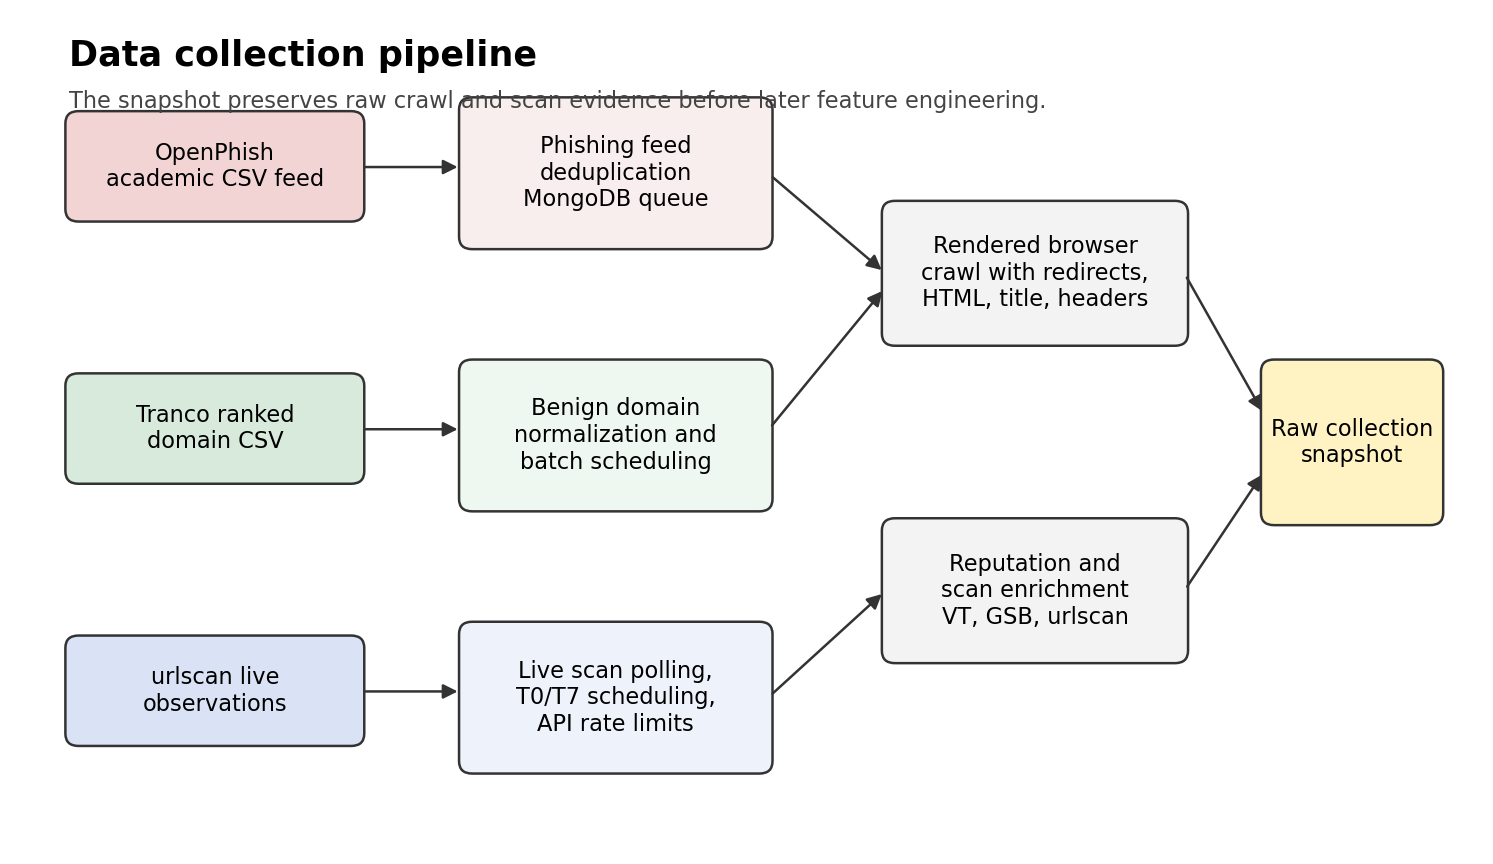
\includegraphics[width=0.92\linewidth]{figures/data_collection_pipeline.png}
\caption{Data collection pipeline before feature engineering.}
\label{fig:data-collection-pipeline}
\end{figure}

Figures~\ref{fig:data-collection-sources} and~\ref{fig:data-collection-labels} summarize the current collection snapshot. The source-count graph is useful for checking whether one acquisition channel dominates the raw corpus. The label-count graph shows the class balance that later stages must account for during splitting and evaluation.

\begin{figure}[htbp]
\centering
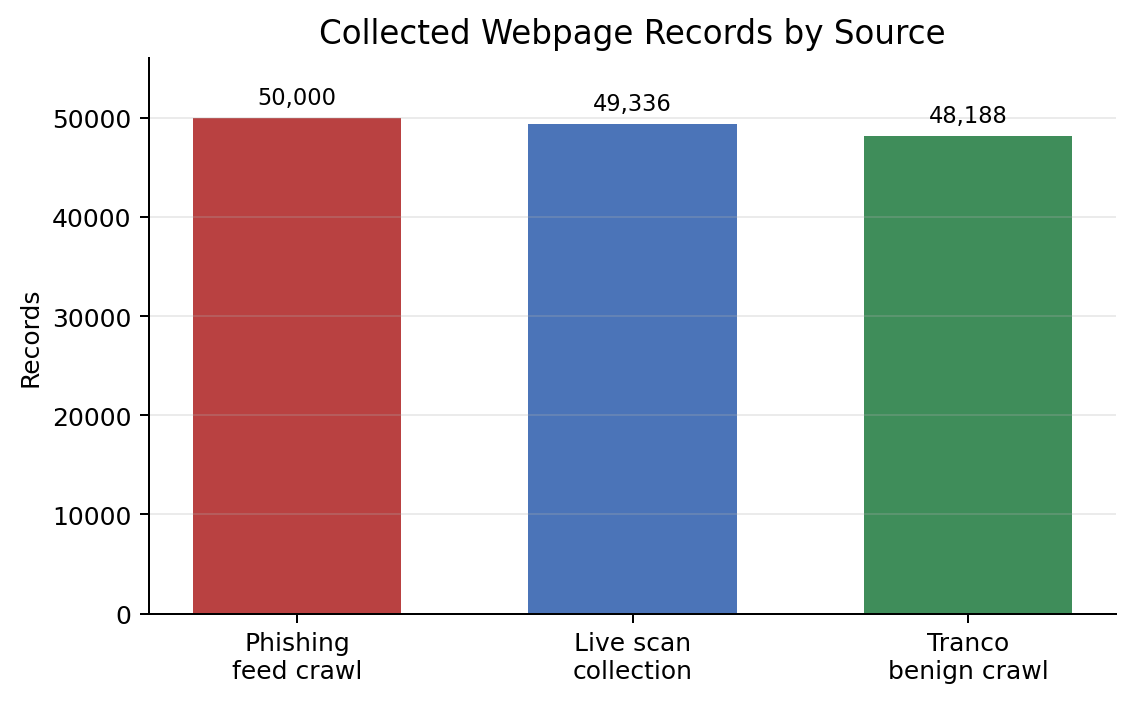
\includegraphics[width=0.72\linewidth]{figures/data_collection_sources.png}
\caption{Record counts by collection source.}
\label{fig:data-collection-sources}
\end{figure}

\begin{figure}[htbp]
\centering
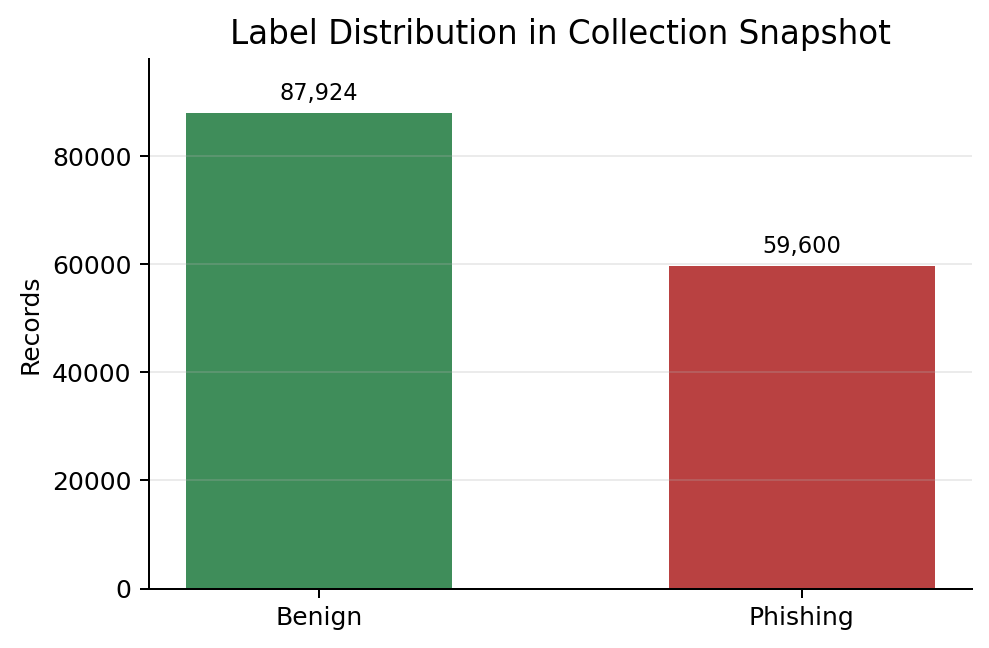
\includegraphics[width=0.62\linewidth]{figures/data_collection_labels.png}
\caption{Label distribution in the current collection snapshot.}
\label{fig:data-collection-labels}
\end{figure}

\subsubsection{Collection Algorithms}
The collection procedures are summarized below as numbered pseudocode. The algorithms describe collection behavior only; feature engineering and model-input construction are intentionally left to the following methodology stage.

\begin{algorithm}[htbp]
\caption{Feed-based phishing webpage collection}
\label{alg:phishing-feed-collection}
\begin{algorithmic}[1]
\Require OpenPhish academic CSV feed, MongoDB connection, polling interval
\Ensure Raw phishing webpage records in \texttt{phishing\_db.website\_content}
\State Poll the OpenPhish academic CSV feed at the configured interval.
\ForAll{rows in the feed}
    \State Parse the row as a candidate phishing URL.
    \If{the URL is not already in the phishing URL queue}
        \State Insert the URL with an \texttt{added\_at} timestamp.
    \EndIf
\EndFor
\State Select URLs that are not marked as visited.
\State Enqueue selected URLs for bounded parallel crawling.
\ForAll{queued URLs}
    \State Open the URL in a headless rendered-browser session.
    \State Wait for DOM loading, network idle, and the configured post-load delay.
    \State Record title, HTML, final URL, status, headers, redirects, timing, and size.
    \State Add RDAP data for the registered domain or IP address.
    \State Store the crawl result, or the crawl error, in the webpage collection.
    \State Mark the source URL as visited with a \texttt{visited\_at} timestamp.
\EndFor
\end{algorithmic}
\end{algorithm}

\begin{algorithm}[htbp]
\caption{Tranco benign webpage collection}
\label{alg:tranco-benign-collection}
\begin{algorithmic}[1]
\Require Tranco CSV file, MongoDB connection, batch size, concurrency limit
\Ensure Raw benign webpage records in \texttt{tranco.websites}
\State Read ranked domains from the Tranco CSV file.
\ForAll{domains in rank order}
    \State Normalize the domain by hostname extraction, lowercasing, and \texttt{www.} removal.
    \If{the normalized domain has already been collected}
        \State Skip the domain.
    \Else
        \State Add the domain to the next crawl batch.
    \EndIf
\EndFor
\ForAll{domains in the batch, using bounded concurrency}
    \State Build HTTPS candidates, trying the \texttt{www} form first for apex domains.
    \ForAll{candidate URLs}
        \State Run HTTP preflight with browser-like headers and redirects enabled.
        \If{preflight status is a non-403 client or server error}
            \State Try the next candidate URL.
        \Else
            \State Open the candidate in a headless rendered-browser session.
            \If{the browser response status is below HTTP 400}
                \State Store title, HTML, final URL, response metadata, redirects, RDAP data, and timestamp.
                \State Stop processing candidates for this domain.
            \EndIf
        \EndIf
    \EndFor
\EndFor
\end{algorithmic}
\end{algorithm}

\begin{algorithm}[htbp]
\caption{Live scan and delayed rescan collection}
\label{alg:live-scan-collection}
\begin{algorithmic}[1]
\Require Live URL observations, VirusTotal keys, optional Safe Browsing and urlscan keys
\Ensure T0 and T7 scan records with pending, completed, failed, and change states
\State Maintain indexes for URL lookup, pending analyses, T7 scheduling, and change flags.
\While{the scanner is running}
    \If{a T7 scrape is pending after significant change}
        \State Perform a bounded follow-up scrape and save the result.
    \ElsIf{an external analysis is pending and ready to poll}
        \State Poll the provider and update the pending scan state.
    \ElsIf{a URL is missing T0 or is due for T7}
        \If{the relevant API rate limiter permits a request}
            \State Submit the scan request and store the pending analysis identifier.
        \EndIf
    \Else
        \State Backfill from live observations until new scan work is available.
    \EndIf
    \State Compare delayed T7 observations with T0 and mark significant changes.
\EndWhile
\end{algorithmic}
\end{algorithm}

\begin{algorithm}[htbp]
\caption{Raw collection snapshot construction}
\label{alg:raw-snapshot-construction}
\begin{algorithmic}[1]
\Require Phishing crawl collection, Tranco crawl collection, live scan collection
\Ensure Auditable raw snapshot for the next methodology stage
\State Read collected records from the phishing, benign, and live-scan collections.
\State Preserve collection source, crawl metadata, scan metadata, and label provenance.
\State Remove exact duplicate observations for the same stored URL and collection state.
\State Count records by source and label for collection auditing.
\State Produce the snapshot totals reported in Table~\ref{tab:data-collection-sources}.
\State Pass the raw snapshot to the next methodology stage.
\end{algorithmic}
\end{algorithm}

\section{RESULTS \& DISCUSSION}
\textit{Give detailed description of the results/achievements including the information:}

\begin{itemize}
\item \textit{To what extent the initial objectives were realized?}
\item \textit{How they differed from the initial objectives?}
\item \textit{Is this project successfully completed?}
\item \textit{Did the project have meaningful contribution to previous state-of-art?}
\item \textit{What is the estimated carbon footprint of the proposed solution (e.g., kg CO\textsubscript{2} eq per functional unit) and how does it compare with conventional alternatives?}
\item \textit{How does the proposed solution perform in terms of economic feasibility when considering cost, supply chain efficiency, and circularity aspects (e.g., reuse, recycling, resource efficiency)?}
\end{itemize}

\section{IMPACT}
\textit{Describe the scientific, technological or socio-economic impacts of your achievements.}

\begin{itemize}
\item \textit{Highlight (if any) innovative and commercial/entrepreneurial aspects of the project.}
\item \textit{Is there any Freedom-to-Use (FTU) issues?}
\item \textit{What are the environmental and sustainability impacts of the proposed solution (e.g., carbon footprint reduction, energy efficiency, resource utilization)?}
\item \textit{How does the solution contribute to circularity and sustainable engineering practices?}
\end{itemize}

\section{ETHICAL ISSUES}
\textit{In this section, you are required to identify (if any) ethical aspects of your project/solution. For instance, are there possible legal/ethical consequences of the solution? Some examples are given below:}

\begin{itemize}
\item \textit{products implicitly using patent protected designs/concepts;}
\item \textit{materials that have better appearance but are toxic}
\item \textit{under design for profit}
\item \textit{products for secret survey of personal private life}
\item \textit{solutions that may have negative affect on health)?}
\end{itemize}

\textit{If there aren't any, you need to still keep this section and state that there are no ethical issues.}

\section{PROJECT MANAGEMENT}
\textit{Initial and final project plans. How, during implementation, project plan has changed and why. What have you learnt in terms of managing your project?}

\section{CONCLUSION AND FUTURE WORK}
\textit{Briefly discuss the most important results/findings of your project. Point out any limitations for your study and conclusions. What are the logical next steps of your project? Provide a short discussion on where the project could go next, if you or other students continued the work. How can the solution be further improved in terms of sustainability, cost efficiency, and real-world implementation?}

\section{APPENDIX}
\textit{Provide, if necessary, additional material such as source code, CAD drawings, proofs of results, etc.}

\section{REFERENCES}
\renewcommand{\refname}{}
\begin{thebibliography}{99}
\bibitem{apwg2025q4} Anti-Phishing Working Group. \textit{Phishing Activity Trends Report, 4th Quarter 2025}. Released December 10, 2025. \url{https://docs.apwg.org/reports/apwg_trends_report_q4_2025.pdf}

\bibitem{tranco2019} V. Le Pochat, T. Van Goethem, S. Tajalizadehkhoob, M. Korczynski, and W. Joosen. ``Tranco: A Research-Oriented Top Sites Ranking Hardened Against Manipulation.'' NDSS, 2019. \url{https://tranco-list.eu/}

\bibitem{openphishacademic} OpenPhish. ``OpenPhish Academic Feed.'' \url{https://github.com/openphish/academic}

\bibitem{virustotaldocs} VirusTotal. ``Analyses Object.'' VirusTotal API Documentation. \url{https://docs.virustotal.com/reference/analyses-object}

\bibitem{urlscandocs} urlscan.io. ``API Documentation.'' \url{https://urlscan.io/docs/api/}

\bibitem{gsbdocs} Google. ``Safe Browsing API v4.'' \url{https://developers.google.com/safe-browsing/v4}

\bibitem{hannousse2021} A. Hannousse and S. Yahiouche. ``Towards Benchmark Datasets for Machine Learning Based Website Phishing Detection: An Experimental Study.'' \textit{Engineering Applications of Artificial Intelligence}, 104:104347, 2021. \url{https://doi.org/10.1016/j.engappai.2021.104347}

\bibitem{aljofey2022} A. Aljofey, Q. Jiang, A. Rasool, H. Chen, W. Liu, Q. Qu, and Y. Wang. ``An Effective Detection Approach for Phishing Websites Using URL and HTML Features.'' \textit{Scientific Reports}, 12:8842, 2022. \url{https://doi.org/10.1038/s41598-022-10841-5}

\bibitem{guo2021} B. Guo, Y. Zhang, C. Xu, F. Shi, Y. Li, and M. Zhang. ``HinPhish: An Effective Phishing Detection Approach Based on Heterogeneous Information Networks.'' \textit{Applied Sciences}, 11(20):9733, 2021. \url{https://doi.org/10.3390/app11209733}

\bibitem{lin2021} Y. Lin, R. Liu, D. M. Divakaran, J. Y. Ng, Q. Z. Chan, Y. Lu, Y. Si, F. Zhang, and J. S. Dong. ``Phishpedia: A Hybrid Deep Learning Based Approach to Visually Identify Phishing Webpages.'' USENIX Security Symposium, 2021. \url{https://www.usenix.org/conference/usenixsecurity21/presentation/lin}

\bibitem{opara2020} C. Opara, B. Wei, and Y. Chen. ``Look Before You Leap: Detecting Phishing Web Pages by Exploiting Raw URL and HTML Characteristics.'' arXiv:2011.04412, 2020. \url{https://arxiv.org/abs/2011.04412}

\bibitem{trad2024} F. Trad and A. Chehab. ``Prompt Engineering or Fine-Tuning? A Case Study on Phishing Detection with Large Language Models.'' \textit{Machine Learning and Knowledge Extraction}, 6(1), 2024. \url{https://www.mdpi.com/2504-4990/6/1/18}

\bibitem{phishllm2024} R. Liu et al. ``Less Defined Knowledge and More True Alarms: Reference-based Phishing Detection without a Pre-defined Reference List.'' USENIX Security Symposium, 2024. \url{https://www.usenix.org/conference/usenixsecurity24/presentation/liu-ruofan}

\bibitem{knowphish2024} Y. Li et al. ``KnowPhish: Large Language Models Meet Multimodal Knowledge Graphs for Enhancing Reference-Based Phishing Detection.'' USENIX Security Symposium, 2024. \url{https://www.usenix.org/conference/usenixsecurity24/presentation/li-yuexin}

\bibitem{phishlang2024} S. S. Roy and S. Nilizadeh. ``PhishLang: A Lightweight, Client-Side Phishing Detection Framework using MobileBERT for Real-Time, Explainable Threat Mitigation.'' arXiv:2408.05667, 2024. \url{https://arxiv.org/abs/2408.05667}

\bibitem{lora2021} E. J. Hu et al. ``LoRA: Low-Rank Adaptation of Large Language Models.'' arXiv:2106.09685, 2021. \url{https://arxiv.org/abs/2106.09685}

\bibitem{qlora2023} T. Dettmers, A. Pagnoni, A. Holtzman, and L. Zettlemoyer. ``QLoRA: Efficient Finetuning of Quantized LLMs.'' NeurIPS, 2023. \url{https://arxiv.org/abs/2305.14314}
\end{thebibliography}

\end{document}
